\section{The Mandelbrot set using OpenMP \punkte{25}}

For this task, I developed two executables. The first, a serial program named \texttt{mandel\_seq.c}, iterates over every pixel in the complex plane, applying the iteration $z \leftarrow z^2 + c$ until either the magnitude of $z$ exceeds 2 or the maximum number of iterations, \texttt{MAX\_ITERS}, is reached. Each pixel's iteration count is stored in a temporary buffer, and a global counter \texttt{nTotalIterationsCount} accumulates the total iterations. The second executable, \texttt{mandel\_par.c}, retains the same computational kernel but parallelizes the pixel loop using \verb|#pragma omp parallel for|. It uses private variables for temporary computations and applies a \verb|reduction(+ : nTotalIterationsCount)| clause to safely sum the iteration counts across threads. To avoid race conditions during image writing, the PNG is generated only after the parallel region completes. A helper script, \texttt{run\_mandel.sh}, automates recompilation of both versions for four image resolutions ($1024^2$, $2048^2$, $4096^2$, and $8192^2$), runs the serial executable once per size, and then executes the OpenMP version with varying thread counts \texttt{OMP\_NUM\_THREADS} set to \{1, 2, 4, 8, 16, 20\}. Each run saves a log file in \texttt{Skeleton\_codes/mandel/logs/} and the corresponding PNG image in \texttt{Skeleton\_codes/mandel/png/}. \\

Example outputs for the two largest resolutions are shown in Figure~\ref{fig:mandel_images}.
\begin{figure}[H]
    \centering
    \begin{subfigure}{0.45\linewidth}
        
\includegraphics[width=\linewidth]{../Skeleton_codes/mandel/png/mandel_4096x4096_T20.png}
        \caption{4096×4096, 20 threads}
    \end{subfigure}
    \hfill
    \begin{subfigure}{0.45\linewidth}
        \includegraphics[width=\linewidth]{../Skeleton_codes/mandel/png/mandel_8192x8192_T20.png}
        \caption{8192×8192, 20 threads}
    \end{subfigure}
    \caption{Mandelbrot renderings generated by the OpenMP version.}
    \label{fig:mandel_images}
\end{figure}

\begin{figure}[H]
    \centering
    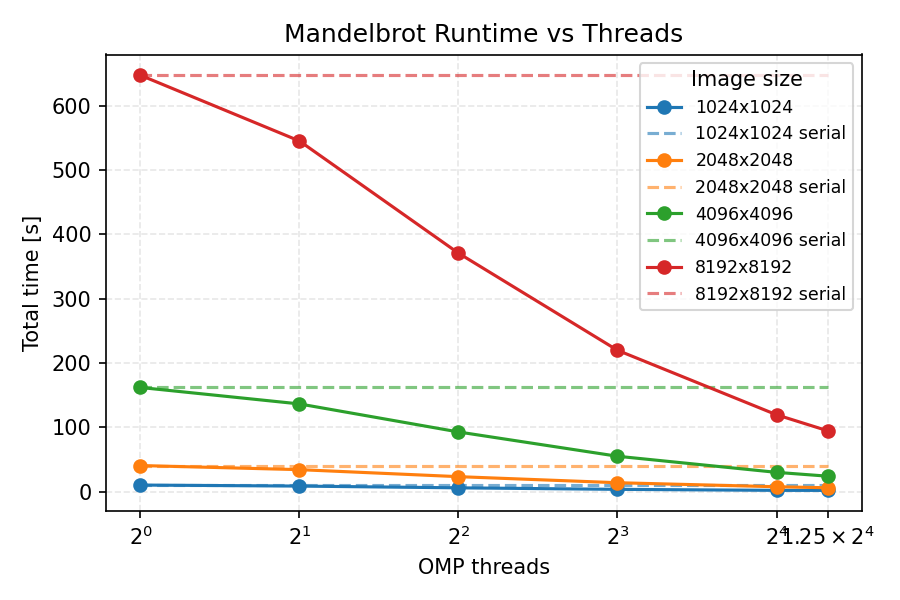
\includegraphics[width=0.75\linewidth]{../Skeleton_codes/mandel/plots/mandel_runtime_scaling.png}
    \caption{Total runtime versus thread count.}
    \label{fig:mandel_scaling}
\end{figure}

Table~\ref{tab:mandel_times} summarises the measured times (seconds) for the OpenMP binary; the serial baseline corresponds to the entry with one thread.
\begin{table}[H]
    \centering
    \begin{tabular}{c|rrrrrr}
        \hline
        Image size & Sequential & 2 threads & 4 threads & 8 threads & 16 threads & 20 threads \\
        \hline
        1024×1024 & 10.13 & 8.54 & 5.80 & 3.44 & 1.88 & 1.80 \\
        2048×2048 & 40.48 & 34.09 & 23.18 & 13.74 & 7.49 & 5.91 \\
        4096×4096 & 161.92 & 136.35 & 92.72 & 54.93 & 29.89 & 23.93 \\
        8192×8192 & 647.71 & 545.44 & 370.92 & 219.81 & 119.51 & 94.57 \\
        \hline
    \end{tabular}
    \caption{Total runtime for the OpenMP version; the iteration count remains constant across threads for each resolution.}
    \label{tab:mandel_times}
\end{table}

Looking at the curves in Figure~\ref{fig:mandel_scaling}, we see that using 20 threads gives us about a 5.6× speedup for the smallest image, and around 6.8× for larger ones. The dashed baselines line up with the measured points when using one thread, so it shows that the OpenMP setup doesn't add any extra overhead outside of the parallel region. For smaller images, the scaling levels off sooner since there’s less work per pixel, and the threads end up competing for memory bandwidth. But when we hit the $8192^2$ resolution, the workload for each thread is bigger, and the speedup stays pretty close to linear. In all cases, the iteration counter and the number of pixels logged match what we expected, which confirms that both the numerical kernel and the performance stats we were asked for are valid.